% =====================================================================
%  Emoji Classification Challenge -- Computer Vision project report
%  Compile with:  pdflatex main.tex  (twice, for the table of contents)
% =====================================================================
\documentclass[11pt,a4paper]{article}

% ---------- packages ----------
\usepackage[T1]{fontenc}
\usepackage[utf8]{inputenc}
\usepackage{lmodern}
\usepackage[english]{babel}
\usepackage{microtype}
\usepackage[a4paper,margin=2.3cm,headheight=14pt]{geometry}
\usepackage{amsmath,amssymb}
\usepackage{graphicx}
\usepackage[table]{xcolor}
\usepackage{booktabs,tabularx,multirow,makecell}
\usepackage{siunitx}
\usepackage{caption,subcaption}
\usepackage{enumitem}
\usepackage{titlesec}
\usepackage{fancyhdr}
\usepackage{float}
\usepackage{listings}
\usepackage{tikz}
\usetikzlibrary{arrows.meta,positioning,fit,calc,shapes.geometric}
\usepackage{pgfplots}
\pgfplotsset{compat=1.18}
\usepackage[most]{tcolorbox}
\usepackage[hidelinks]{hyperref}

% ---------- colours & style ----------
\definecolor{navy}{HTML}{0B2D5B}
\definecolor{accent}{HTML}{2E6DB4}
\definecolor{soft}{HTML}{EAF1FA}
\definecolor{good}{HTML}{2E7D32}
\definecolor{bad}{HTML}{C62828}
\definecolor{grey}{HTML}{6B7280}

\hypersetup{colorlinks=true,linkcolor=navy,citecolor=accent,urlcolor=accent}
\captionsetup{font=small,labelfont={bf,color=navy},format=hang}
\setlist{itemsep=2pt,topsep=4pt}
\sisetup{detect-weight=true,group-minimum-digits=4}

\titleformat{\section}{\Large\bfseries\sffamily\color{navy}}{\thesection}{0.8em}{}[{\color{accent}\titlerule[0.8pt]}]
\titleformat{\subsection}{\large\bfseries\sffamily\color{navy}}{\thesubsection}{0.8em}{}
\titleformat{\subsubsection}{\normalsize\bfseries\sffamily\color{accent}}{\thesubsubsection}{0.8em}{}
\titlespacing*{\section}{0pt}{18pt}{10pt}

\pagestyle{fancy}
\fancyhf{}
\fancyhead[L]{\small\sffamily\color{grey}Emoji Classification Challenge}
\fancyhead[R]{\small\sffamily\color{grey}Computer Vision -- ESSEC 2026/27}
\fancyfoot[C]{\small\sffamily\thepage}
\renewcommand{\headrulewidth}{0.4pt}

\newtcolorbox{keybox}[1][]{enhanced,colback=soft,colframe=accent,boxrule=0.6pt,
  arc=2pt,left=8pt,right=8pt,top=6pt,bottom=6pt,fonttitle=\bfseries\sffamily,
  coltitle=white,colbacktitle=accent,#1}

\lstset{basicstyle=\ttfamily\footnotesize,backgroundcolor=\color{soft},frame=single,
  rulecolor=\color{accent},framerule=0.4pt,breaklines=true,columns=fullflexible,
  keywordstyle=\color{navy}\bfseries,commentstyle=\color{grey}\itshape,
  stringstyle=\color{good},language=Python,showstringspaces=false,xleftmargin=4pt,xrightmargin=4pt}

\newcommand{\code}[1]{\texttt{\small #1}}
\newcommand{\vendor}[1]{\textsf{#1}}
\newcommand{\up}[1]{\textcolor{good}{#1}}
\newcommand{\down}[1]{\textcolor{bad}{#1}}

% ---------- Kaggle leaderboard (not stored in the repository) ----------
\newcommand{\kagglepublic}{0.98238}

% =====================================================================
\begin{document}

% ============================ 1. FRONT PAGE ============================
\begin{titlepage}
\thispagestyle{empty}
\newgeometry{margin=2.3cm}
\begin{tikzpicture}[remember picture,overlay]
  \fill[navy] (current page.north west) rectangle ([yshift=-6.2cm]current page.north east);
  \fill[accent] ([yshift=-6.2cm]current page.north west) rectangle ([yshift=-6.4cm]current page.north east);
\end{tikzpicture}

\vspace*{-0.6cm}
{\color{white}\sffamily
  {\large ESSEC Business School \hfill Computer Vision -- 2026/2027}\\[1.1cm]
  {\fontsize{30}{36}\selectfont\bfseries Emoji Classification Challenge}\\[0.35cm]
  {\Large Recognising the vendor style of an emoji with a fine-tuned ConvNeXt}
}

\vspace{2.6cm}
\begin{center}
  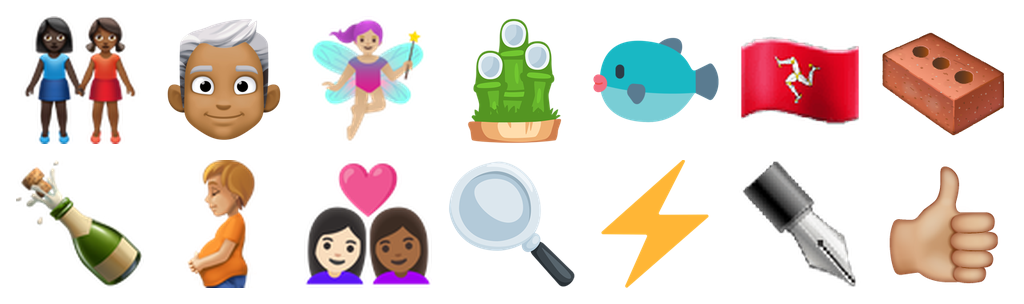
\includegraphics[width=0.95\textwidth]{figures/banner.png}\\[0.2cm]
  {\small\color{grey}One column per vendor, from left to right: \vendor{apple}, \vendor{facebook},
  \vendor{google}, \vendor{messenger}, \vendor{mozilla}, \vendor{samsung}, \vendor{whatsapp}.}
\end{center}

\vspace{1.4cm}
\begin{center}
\begin{tcolorbox}[enhanced,width=0.82\textwidth,colback=soft,colframe=accent,boxrule=0.6pt,arc=2pt,
  left=10pt,right=10pt,top=8pt,bottom=8pt]
\sffamily
\begin{tabularx}{\linewidth}{@{}l X@{}}
  \textbf{Task}          & 7-class image classification (emoji vendor) \\
  \textbf{Model}         & ConvNeXt-Tiny (CNN), ImageNet-22k pretrained, 5-fold ensemble \\
  \textbf{Validation}    & Out-of-fold accuracy \textbf{97.56\,\%}, macro-F1 \textbf{0.976} \\
  \textbf{Leaderboard}   & Kaggle public score \textbf{\kagglepublic} \\
  \textbf{Deliverables}  & \code{emoji\_classifier.ipynb}, \code{submission.csv}, this report \\
\end{tabularx}
\end{tcolorbox}
\end{center}

\vfill
{\sffamily
\begin{center}
  {\large\bfseries Team}\\[0.25cm]
  {\large Augustin \quad$\cdot$\quad Gabriel \quad$\cdot$\quad Nicolas \quad$\cdot$\quad Raphaël}\\[0.5cm]
  {\color{grey} October 2026}
\end{center}}
\restoregeometry
\end{titlepage}

% ====================== 2. ABSTRACT + TOC + MODEL ======================
\section*{Abstract}
\addcontentsline{toc}{section}{Abstract}

We address the \emph{Emoji Classification Challenge}: given an emoji image, predict which of seven
vendors (\vendor{apple}, \vendor{facebook}, \vendor{google}, \vendor{messenger}, \vendor{mozilla},
\vendor{samsung}, \vendor{whatsapp}) drew it. The training set contains \num{9879} labelled PNG files
and the test set \num{9879} unlabelled ones. The difficulty is not \emph{what} is drawn, since every vendor
draws the same objects, but \emph{how} it is drawn: line weight, shading, palette, margins and
anti-aliasing.

Our solution is a \textbf{convolutional neural network}, \textbf{ConvNeXt-Tiny}
(\num{27.8}\,M parameters) pretrained on ImageNet-22k and fine-tuned end to end on $160\times160$ inputs.
Most of the work went into the input pipeline. Every PNG colour mode is decoded to \emph{premultiplied}
RGBA, padded to a square, resized and composited on white. This removes colour information that is
hidden under transparent pixels and differs between vendors. Exact duplicates are found with a pixel
fingerprint and kept inside one fold of a \emph{stratified group} 5-fold cross-validation, so the validation
score is not inflated. An ablation study showed that the usual geometric data augmentation
\emph{lowers} accuracy by 2.7 points, so the final model is trained without augmentation.

The 5-fold ensemble reaches an out-of-fold accuracy of \textbf{97.56\,\%} and a macro-F1 of
\textbf{0.976}, against 66.7\,\% for a baseline that only reads file metadata, and its submission scores
\textbf{\kagglepublic} on the Kaggle public leaderboard. The remaining errors
are concentrated on the 4.5\,\% of images delivered at an unusual (small) resolution: they account for
45\,\% of the mistakes.

\vspace{0.4cm}
\begin{keybox}[title={Model chosen at a glance}]
\begin{tabularx}{\linewidth}{@{}>{\bfseries}l X@{}}
Family        & \textbf{CNN}: supervised convolutional network, \emph{not} a Vision-Language Model (VLM) nor a pure Vision Transformer. \\
Backbone      & ConvNeXt-Tiny \cite{liu2022convnext}, \code{timm} weights \code{convnext\_tiny.fb\_in22k\_ft\_in1k}. \\
Head          & Global average pooling $\rightarrow$ LayerNorm $\rightarrow$ linear layer $768\rightarrow7$ (new, randomly initialised). \\
Learning      & Transfer learning: full fine-tuning, AdamW, one-cycle cosine schedule, label smoothing. \\
Inference     & Average of the 5 fold models' softmax outputs, then an exact-duplicate lookup. \\
\end{tabularx}
\end{keybox}

\newpage
\tableofcontents
\newpage

% ============================ INTRODUCTION ============================
\section{Introduction and choice of model}
\label{sec:intro}

\subsection{The task}
Each image of the challenge is one emoji rendered by one of seven vendors. The label is the vendor, not
the emoji: a ``frog'' drawn by Apple and a ``frog'' drawn by Google belong to two different classes,
while a frog and a car drawn by Google belong to the same class. A classifier therefore has to ignore the
semantic content and focus on the \emph{graphic style}. Figure~\ref{fig:samples} shows random training
images per vendor. Some styles are easy to recognise (Mozilla's flat design, Samsung's glossy look),
others are close to each other (Facebook and Messenger, two Meta products).

\begin{figure}[H]
  \centering
  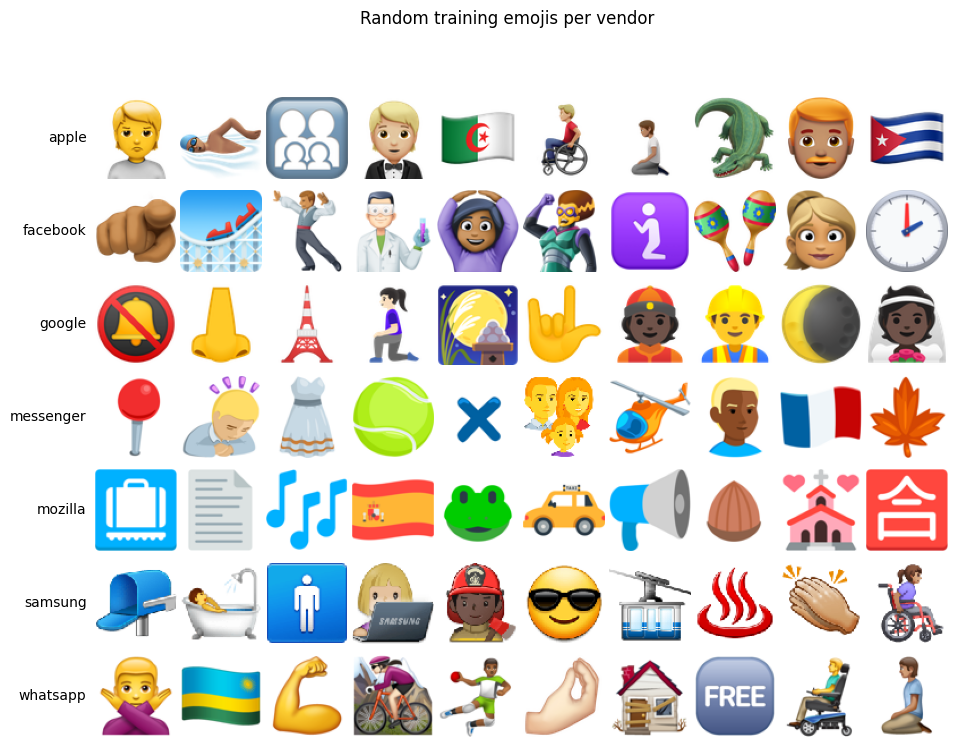
\includegraphics[width=0.78\textwidth,trim=0 0 0 60,clip]{figures/samples_grid.png}
  \caption{Ten random training emojis per vendor (composited on white). The class is the drawing style,
  not the object.}
  \label{fig:samples}
\end{figure}

The submission is a CSV file with columns \code{Id,Label} for the \num{9879} test images.

\subsection{Why a CNN, and why ConvNeXt?}
We considered three families of models.

\begin{itemize}
  \item \textbf{Vision-Language Models (CLIP-like, or generative VLMs).} They are trained to match
  images with captions, so their features describe \emph{what} is in the image (``a green frog'') and
  are, by design, fairly invariant to rendering style. Zero-shot prompts such as ``an Apple emoji'' would
  rely on knowledge the model is unlikely to have at the pixel level, and a VLM is also much heavier to run
  on \num{9879} test images. The task does not need language.
  \item \textbf{Vision Transformers.} They are competitive when pretrained at scale, but they work on
  $16\times16$ patches and have weaker locality priors. On a dataset of about \num{10000} images and at a
  low input resolution, a CNN is usually easier to fine-tune.
  \item \textbf{Convolutional networks.} Their inductive biases (local filters, weight sharing,
  translation equivariance) fit what separates vendors: edge sharpness, anti-aliasing, gradients and
  textures. They are also cheap enough to train a 5-fold ensemble on a laptop GPU.
\end{itemize}

We chose \textbf{ConvNeXt-Tiny} \cite{liu2022convnext}, a ``modernised'' CNN that brings design choices
of Vision Transformers (patchify stem, large $7\times7$ depthwise kernels, LayerNorm, GELU, inverted
bottlenecks) into a pure convolutional network. Its ImageNet-22k pretraining (about 14\,M images
\cite{deng2009imagenet}) gives very good transfer to small datasets. During exploration we also tried
224\,px inputs, 15 epochs, ConvNeXt-Small and EfficientNetV2-S on a single fold: none improved on
ConvNeXt-Tiny at 160\,px by more than the noise level, and they cost $1.5$ to $2\times$ more training time.

\subsection{Overview of the pipeline}
Figure~\ref{fig:pipeline} summarises the full pipeline, which the next sections describe step by step.

\begin{figure}[H]
\centering
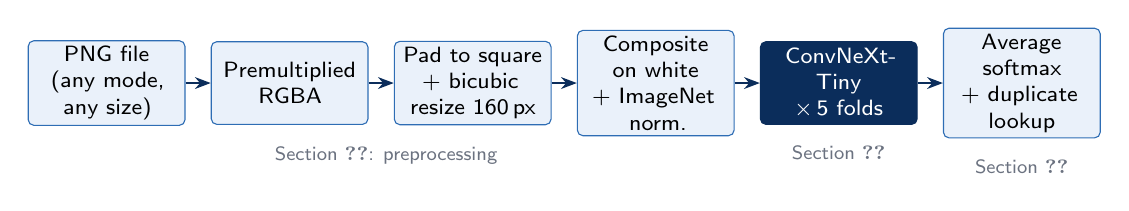
\begin{tikzpicture}[
  node distance=0.32cm and 0.32cm,
  box/.style={draw=accent,fill=soft,rounded corners=2pt,align=center,font=\footnotesize\sffamily,
              minimum height=1.05cm,text width=1.85cm,inner sep=2pt},
  mbox/.style={box,fill=navy,text=white,draw=navy},
  arr/.style={-{Stealth[length=2mm]},thick,color=navy}]
  \node[box] (png) {PNG file\\(any mode, any size)};
  \node[box,right=of png] (pre) {Premultiplied RGBA};
  \node[box,right=of pre] (pad) {Pad to square\\+ bicubic resize 160\,px};
  \node[box,right=of pad] (white) {Composite on white\\+ ImageNet norm.};
  \node[mbox,right=of white] (net) {ConvNeXt-Tiny\\$\times$\,5 folds};
  \node[box,right=of net] (avg) {Average softmax\\+ duplicate lookup};
  \draw[arr] (png)--(pre); \draw[arr] (pre)--(pad); \draw[arr] (pad)--(white);
  \draw[arr] (white)--(net); \draw[arr] (net)--(avg);
  \node[font=\scriptsize\sffamily\color{grey},below=0.15cm of pad,xshift=-1.1cm] {Section~\ref{sec:prepro}: preprocessing};
  \node[font=\scriptsize\sffamily\color{grey},below=0.15cm of net] {Section~\ref{sec:archi}};
  \node[font=\scriptsize\sffamily\color{grey},below=0.15cm of avg] {Section~\ref{sec:perf}};
\end{tikzpicture}
\caption{End-to-end pipeline, from a raw PNG file to the predicted vendor.}
\label{fig:pipeline}
\end{figure}

% ============================ PREPROCESSING ============================
\section{Preprocessing}
\label{sec:prepro}

\subsection{Exploring the data}

\paragraph{Class balance.} The classes are imbalanced (Table~\ref{tab:data}): \vendor{mozilla} (397
images) and \vendor{messenger} (580) are four to five times rarer than \vendor{apple} (\num{1924}).
This is why we report the \textbf{macro-F1} next to accuracy (Section~\ref{sec:metrics}) and use
\emph{stratified} folds.

\paragraph{The files are not uniform.} Unlike MNIST-style datasets, the images come in eight native sizes
and five PNG colour modes, and both are strongly tied to the vendor (Table~\ref{tab:data}). For example,
almost all \vendor{whatsapp} images are $160\times160$, while \vendor{facebook}, \vendor{messenger} and
\vendor{mozilla} are mostly $240\times240$, and \vendor{apple}, \vendor{google} and \vendor{samsung} are
mostly $72\times72$. \vendor{samsung} is the only vendor that mostly uses palette (\code{P}) images.

\begin{table}[H]
\centering
\small
\caption{Training set per vendor: number of images, most frequent native size and PNG colour mode
(with the share of the vendor's images they represent).}
\label{tab:data}
\begin{tabular}{l S[table-format=4.0] S[table-format=3.1] l l}
\toprule
\textbf{Vendor} & {\textbf{Images}} & {\textbf{Share (\%)}} & \textbf{Main native size} & \textbf{Main PNG mode} \\
\midrule
\vendor{apple}     & 1924 & 19.5 & $72\times72$ (99.9\,\%)   & RGBA (93.9\,\%) \\
\vendor{facebook}  & 1667 & 16.9 & $240\times240$ (93.0\,\%) & RGBA (99.0\,\%) \\
\vendor{google}    & 1877 & 19.0 & $72\times72$ (93.6\,\%)   & RGBA (98.0\,\%) \\
\vendor{messenger} &  580 &  5.9 & $240\times240$ (98.6\,\%) & RGBA (99.5\,\%) \\
\vendor{mozilla}   &  397 &  4.0 & $240\times240$ (91.2\,\%) & RGBA (95.2\,\%) \\
\vendor{samsung}   & 1790 & 18.1 & $72\times72$ (99.7\,\%)   & P (88.3\,\%) \\
\vendor{whatsapp}  & 1644 & 16.6 & $160\times160$ (90.3\,\%) & RGBA (96.9\,\%) \\
\midrule
\textbf{Total}     & 9879 & 100.0 & \multicolumn{2}{l}{8 native sizes, 5 PNG modes (RGBA, P, LA, RGB, L)} \\
\bottomrule
\end{tabular}
\end{table}

\paragraph{A metadata-only baseline.} To measure how much these file properties reveal, we trained a
decision tree on the one-hot encoded native size and colour mode only, without reading a single pixel.
Evaluated with the same folds as the CNN, it reaches \textbf{66.7\,\%} accuracy but only \textbf{0.486}
macro-F1: it cannot separate the many $72\times72$ RGBA images, nor the $240\times240$ vendors. It is a
shortcut, not the visual style we are asked to recognise, so the network below receives \emph{pixels
only}: every image is brought to the same square size and the same background. (The original resolution
remains indirectly visible, because a 72\,px image upscaled to 160\,px is blurrier. This cannot be avoided.)

\subsection{Careful decoding of transparency}
\label{sec:alpha}

\paragraph{The problem: hidden colours.} All files are PNGs with transparency (RGBA, palette with a
transparent index, grey-scale with alpha\ldots). A fully transparent pixel is invisible, \emph{but it
still stores an RGB value}, and that value depends on the software each vendor used to export its
images. Table~\ref{tab:hidden} gives the mean colour stored under fully transparent pixels. The common
call \code{Image.open(f).convert("RGB")} simply drops the alpha channel and exposes these colours to the
network (top row of Figure~\ref{fig:alpha}).

\begin{table}[H]
\centering\small
\caption{Mean RGB value stored under fully transparent pixels ($\alpha=0$), over 200 training images per
vendor. Samsung hides a grey-blue colour, Mozilla almost pure black.}
\label{tab:hidden}
\begin{tabular}{l *{7}{S[table-format=3.1]}}
\toprule
 & {\vendor{apple}} & {\vendor{facebook}} & {\vendor{google}} & {\vendor{messenger}} & {\vendor{mozilla}} & {\vendor{samsung}} & {\vendor{whatsapp}} \\
\midrule
Mean R & 42.1 & 80.8 & 29.2 & 36.6 & 8.9 & 71.6 & 64.9 \\
Mean G & 36.3 & 65.7 & 26.0 & 29.9 & 8.9 & 97.7 & 52.2 \\
Mean B & 28.6 & 57.1 & 20.8 & 24.8 & 8.5 & 100.3 & 42.4 \\
\bottomrule
\end{tabular}
\end{table}

\begin{figure}[H]
  \centering
  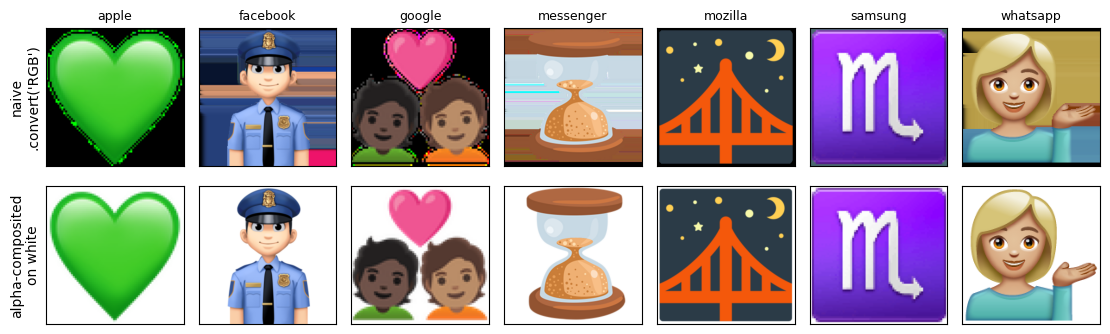
\includegraphics[width=0.92\textwidth]{figures/naive_vs_composited.png}
  \caption{Top: naive conversion to RGB, where the hidden colours under transparent pixels become
  visible (black, stripes, coloured backgrounds). Bottom: our preprocessing, alpha-composited on
  white.}
  \label{fig:alpha}
\end{figure}

These hidden colours are a potential \textbf{shortcut}: a network could learn ``grey-blue background
$\Rightarrow$ samsung'' instead of the drawing style, and such a rule would break as soon as the images
are exported by another tool. We remove it with \textbf{premultiplied alpha} \cite{porter1984compositing}.

\paragraph{Our decoding pipeline.} For every file (function \code{load\_premultiplied}):
\begin{enumerate}
  \item convert any mode (\code{RGBA}, \code{P}, \code{LA}, \code{L}, \code{RGB}) to RGBA with values
  $c\in[0,1]^3$ and $\alpha\in[0,1]$;
  \item \textbf{premultiply} the colour by the opacity:
  \begin{equation}
    \tilde c = \alpha\, c .
  \end{equation}
  Hidden colours under $\alpha=0$ become exactly $0$, and semi-transparent edge pixels are weighted
  correctly;
  \item \textbf{pad} non-square images (e.g.\ $72\times68$) with transparent pixels, centred, so that
  they are not distorted;
  \item \textbf{resize} to $160\times160$ with an anti-aliased bicubic filter. Resizing premultiplied
  colours avoids the dark or coloured halos that appear when straight RGBA is resized. Because bicubic
  interpolation can overshoot, we clamp $0\le\tilde c\le\alpha$;
  \item store the 4-channel result as \code{uint8} in memory (about 1\,GB each for train and test);
  \item at batch time, on the GPU, \textbf{composite on white}:
  \begin{equation}
    \text{rgb} = \tilde c + (1-\alpha)\cdot \mathbf 1 ,
  \end{equation}
  then standardise with the ImageNet statistics used during pretraining,
  $x = (\text{rgb}-\mu)/\sigma$ with $\mu=(0.485,0.456,0.406)$ and $\sigma=(0.229,0.224,0.225)$.
\end{enumerate}
We checked that after compositing, every fully transparent pixel has the value $1.0$ (pure white) for
every vendor. Figure~\ref{fig:input} shows what the network actually receives.

\begin{figure}[H]
  \centering
  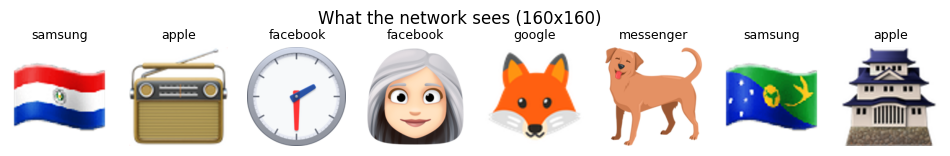
\includegraphics[width=0.92\textwidth,trim=0 0 0 22,clip]{figures/network_input.png}
  \caption{Network inputs after preprocessing ($160\times160$, premultiplied, composited on white).}
  \label{fig:input}
\end{figure}

\subsection{Exact duplicates and honest validation folds}
\label{sec:dups}

During decoding we compute a \textbf{fingerprint} of each image: an MD5 hash of its native-resolution
premultiplied pixels (plus its shape). Two files share a fingerprint exactly when they look identical;
hidden colours are ignored. This revealed that:
\begin{itemize}
  \item the training set holds \num{9721} distinct images: \textbf{141 duplicate groups} cover 299
  files. They are mostly people emojis whose default and gendered versions (e.g.\ \emph{detective} and
  \emph{man detective}) are drawn identically by the vendor;
  \item the copies of an image \textbf{always carry the same label} (0 conflicting groups);
  \item \textbf{352 test images} are pixel-identical to at least one training image.
\end{itemize}
If two copies of the same image fell into different folds, the model would be validated on an image it
had already seen, and the validation score would be optimistic. We therefore build the 5 folds with
\code{StratifiedGroupKFold}, using the fingerprint as the group: all copies of an image stay in the same
fold, and each fold keeps the class proportions (\num{7903} training and \num{1976} validation images per
fold). The code asserts that no fingerprint is shared between the training and validation parts of a fold.

\subsection{Data augmentation: a measured decision to use none}
\label{sec:augm}

Data augmentation is usually essential on a dataset of this size. Here we tested it and decided
\textbf{not} to use it. The code still contains the augmentations, run on the GPU and switched on with
configuration flags, so that the ablation (Section~\ref{sec:ablation}) can be reproduced:

\begin{itemize}
  \item \textbf{Geometric augmentation} (\code{geometric\_aug}): random rotation of $\pm10^\circ$, zoom
  in $[0.85,1.15]$ and translation of $\pm8\,\%$, applied with one affine transform per image and
  bilinear resampling. The border is filled with white by computing $1-\text{grid\_sample}(1-x)$.
  Result: \down{$-2.7$ accuracy points}.
  \item \textbf{Horizontal flip} (\code{hflip}, plus flip test-time augmentation \code{tta\_hflip}): an
  exact mirror, with no resampling. Result: no measurable effect (97.52\,\% vs 97.56\,\% OOF accuracy
  over the full 5-fold cross-validation).
  \item \textbf{Colour jitter}: excluded by design, because the colour palette is part of a vendor's
  style.
\end{itemize}

\begin{keybox}[title={Why augmentation hurts here}]
Each vendor draws its emojis on a fixed canvas, with consistent margins, size and position, and
renders them with crisp, vendor-specific anti-aliasing. Rotating or zooming resamples the image, which
shifts and blurs exactly these cues. Unlike natural photos, the test images come from the same rendering
process as the training images, so there is no viewpoint variation for augmentation to cover.
\end{keybox}

% ============================ ARCHITECTURE ============================
\section{Architecture of the model}
\label{sec:archi}

\subsection{ConvNeXt-Tiny}

ConvNeXt \cite{liu2022convnext} starts from a ResNet and modernises it step by step with ideas from
Vision Transformers. The Tiny variant has four stages with $(3,3,9,3)$ blocks and $(96,192,384,768)$
channels. Figure~\ref{fig:archi} gives the full network for our $160\times160$ inputs, with the shape of
the feature maps after each stage.

\begin{figure}[H]
\centering
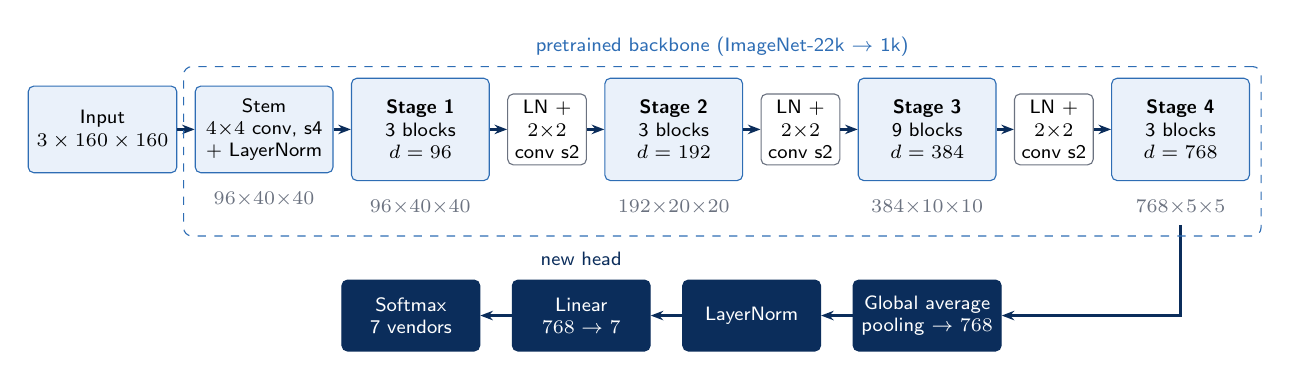
\begin{tikzpicture}[
  node distance=0.22cm,
  st/.style={draw=accent,fill=soft,rounded corners=2pt,align=center,font=\scriptsize\sffamily,
             minimum width=1.75cm,inner sep=3pt},
  ds/.style={draw=grey,fill=white,rounded corners=2pt,align=center,font=\scriptsize\sffamily,
             minimum width=1.0cm,inner sep=2pt},
  hd/.style={st,fill=navy,text=white,draw=navy},
  arr/.style={-{Stealth[length=1.6mm]},thick,color=navy},
  shp/.style={font=\scriptsize\sffamily\color{grey}}]
  \node[st,minimum height=1.1cm] (in) {Input\\$3\times160\times160$};
  \node[st,right=of in,minimum height=1.1cm] (stem) {Stem\\$4{\times}4$ conv, s4\\+ LayerNorm};
  \node[st,right=of stem,minimum height=1.3cm] (s1) {\textbf{Stage 1}\\3 blocks\\$d=96$};
  \node[ds,right=of s1,minimum height=0.9cm] (d1) {LN +\\$2{\times}2$\\conv s2};
  \node[st,right=of d1,minimum height=1.3cm] (s2) {\textbf{Stage 2}\\3 blocks\\$d=192$};
  \node[ds,right=of s2,minimum height=0.9cm] (d2) {LN +\\$2{\times}2$\\conv s2};
  \node[st,right=of d2,minimum height=1.3cm] (s3) {\textbf{Stage 3}\\9 blocks\\$d=384$};
  \node[ds,right=of s3,minimum height=0.9cm] (d3) {LN +\\$2{\times}2$\\conv s2};
  \node[st,right=of d3,minimum height=1.3cm] (s4) {\textbf{Stage 4}\\3 blocks\\$d=768$};
  \foreach \a/\b in {in/stem,stem/s1,s1/d1,d1/s2,s2/d2,d2/s3,s3/d3,d3/s4} \draw[arr] (\a)--(\b);
  \node[shp,below=0.12cm of stem] (sh0) {$96{\times}40{\times}40$};
  \node[shp,below=0.12cm of s1] (sh1) {$96{\times}40{\times}40$};
  \node[shp,below=0.12cm of s2] (sh2) {$192{\times}20{\times}20$};
  \node[shp,below=0.12cm of s3] (sh3) {$384{\times}10{\times}10$};
  \node[shp,below=0.12cm of s4] (sh4) {$768{\times}5{\times}5$};
  % head
  \node[hd,below=1.25cm of s3,minimum height=0.9cm] (gap) {Global average\\pooling $\to 768$};
  \node[hd,left=0.4cm of gap,minimum height=0.9cm] (ln) {LayerNorm};
  \node[hd,left=0.4cm of ln,minimum height=0.9cm] (fc) {Linear\\$768\to7$};
  \node[hd,left=0.4cm of fc,minimum height=0.9cm] (sm) {Softmax\\7 vendors};
  \draw[arr] (sh4.south) |- (gap.east);
  \draw[arr] (gap)--(ln); \draw[arr] (ln)--(fc); \draw[arr] (fc)--(sm);
  \node[font=\scriptsize\sffamily\color{navy},above=0.05cm of fc] {new head};
  \node[draw=accent,dashed,rounded corners=3pt,fit=(stem)(s4)(sh0)(sh4),inner sep=4pt,
        label={[font=\scriptsize\sffamily\color{accent}]above:pretrained backbone (ImageNet-22k $\to$ 1k)}] {};
\end{tikzpicture}
\caption{ConvNeXt-Tiny on a $160\times160$ input. The backbone downsamples by 32 in total, so the last
stage works on a $5\times5$ grid; a new 7-way classification head replaces the 1000-class ImageNet head.}
\label{fig:archi}
\end{figure}

\paragraph{The ConvNeXt block.} Every block of a stage has the same structure (Figure~\ref{fig:block}).
With $x$ a $d$-channel feature map:
\begin{equation}
  y = x + \gamma\odot\operatorname{Linear}_{4d\to d}\!\Big(\operatorname{GELU}\big(\operatorname{Linear}_{d\to4d}(\operatorname{LN}(\operatorname{DWConv}_{7\times7}(x)))\big)\Big),
\end{equation}
where $\gamma$ is a learned per-channel \emph{layer scale}. The design choices that come from Transformers are:
\begin{itemize}
  \item a \textbf{$7\times7$ depthwise convolution} mixes information spatially, channel by channel,
  with a large receptive field (similar to the local attention window of a Swin Transformer);
  \item an \textbf{inverted bottleneck} ($d\to4d\to d$, implemented as $1\times1$ convolutions /
  linear layers) mixes the channels, like the MLP of a Transformer block;
  \item a single \textbf{LayerNorm} and a single \textbf{GELU} per block, instead of BatchNorm and ReLU
  after every convolution;
  \item a \textbf{patchify stem} ($4\times4$ convolution with stride 4) and \textbf{separate
  downsampling layers} between stages.
\end{itemize}

\begin{figure}[H]
\centering
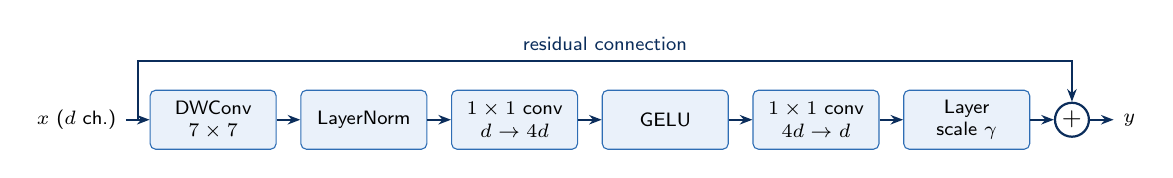
\begin{tikzpicture}[
  node distance=0.3cm,
  b/.style={draw=accent,fill=soft,rounded corners=2pt,font=\scriptsize\sffamily,align=center,
            minimum height=0.75cm,minimum width=1.6cm},
  arr/.style={-{Stealth[length=1.6mm]},thick,color=navy}]
  \node[font=\scriptsize\sffamily] (x) {$x$ ($d$ ch.)};
  \node[b,right=of x] (dw) {DWConv\\$7\times7$};
  \node[b,right=of dw] (ln) {LayerNorm};
  \node[b,right=of ln] (f1) {$1\times1$ conv\\$d\to4d$};
  \node[b,right=of f1] (ge) {GELU};
  \node[b,right=of ge] (f2) {$1\times1$ conv\\$4d\to d$};
  \node[b,right=of f2] (ls) {Layer\\scale $\gamma$};
  \node[circle,draw=navy,thick,right=of ls,inner sep=1pt,font=\small] (plus) {$+$};
  \node[font=\scriptsize\sffamily,right=of plus] (y) {$y$};
  \foreach \a/\b in {x/dw,dw/ln,ln/f1,f1/ge,ge/f2,f2/ls,ls/plus,plus/y} \draw[arr] (\a)--(\b);
  \draw[arr] ([xshift=-0.15cm]dw.west) -- ++(0,0.75) -| (plus.north)
    node[pos=0.25,above,font=\scriptsize\sffamily\color{grey}] {residual connection};
\end{tikzpicture}
\caption{A ConvNeXt block (stochastic depth is disabled in our configuration).}
\label{fig:block}
\end{figure}

\paragraph{Size of the model.} Table~\ref{tab:params} breaks down the \num{27825511} parameters. Almost
all of them are pretrained: the head has \num{6919} parameters, and only the \num{5383} of its final linear layer are new. Because the network is
fully convolutional and ends with a global pooling, it accepts our 160\,px inputs even though it was
pretrained at 224\,px.

\begin{table}[H]
\centering\small
\caption{Parameters of ConvNeXt-Tiny with a 7-class head (stage counts include the downsampling layer in
front of the stage).}
\label{tab:params}
\begin{tabular}{l l S[table-format=8.0] S[table-format=3.2]}
\toprule
\textbf{Part} & \textbf{Output shape (160\,px input)} & {\textbf{Parameters}} & {\textbf{Share (\%)}} \\
\midrule
Stem                  & $96\times40\times40$   & 4896     & 0.02 \\
Stage 1 (3 blocks)    & $96\times40\times40$   & 237888   & 0.85 \\
Stage 2 (3 blocks)    & $192\times20\times20$  & 992256   & 3.57 \\
Stage 3 (9 blocks)    & $384\times10\times10$  & 11112960 & 39.94 \\
Stage 4 (3 blocks)    & $768\times5\times5$    & 15470592 & 55.60 \\
Head (LN + linear)    & $7$                    & 6919     & 0.02 \\
\midrule
\textbf{Total}        &                        & 27825511 & 100.00 \\
\bottomrule
\end{tabular}
\end{table}

\subsection{Transfer learning and training procedure}

We use the \code{timm} \cite{wightman2019timm} weights \code{convnext\_tiny.fb\_in22k\_ft\_in1k}
(pretrained on ImageNet-22k, then fine-tuned on ImageNet-1k). \code{timm} replaces the classifier by a
randomly initialised 7-way linear layer, and the \emph{whole} network is then fine-tuned.
Table~\ref{tab:hyper} lists the hyper-parameters.

\begin{table}[H]
\centering\small
\caption{Training configuration (the \code{CFG} dictionary of the notebook).}
\label{tab:hyper}
\begin{tabularx}{0.92\textwidth}{@{}l l X@{}}
\toprule
\textbf{Setting} & \textbf{Value} & \textbf{Comment} \\
\midrule
Input size        & $160\times160$ & At least the native size of every image except the $240\times240$ ones; cheaper than 224 at no measurable loss \\
Batch size        & 64             & 123 steps per epoch (incomplete last batch dropped) \\
Epochs            & 12             & \num{1476} optimisation steps per fold \\
Optimiser         & AdamW \cite{loshchilov2019adamw} & learning rate $3\cdot10^{-4}$, weight decay $0.05$ \\
LR schedule       & One-cycle \cite{smith2019superconvergence} & linear warm-up from $\text{lr}/25$ over the first 10\,\% of steps, then cosine decay to $\approx0$; $\beta_1$ cycled between $0.95$ and $0.85$ \\
Loss              & Cross-entropy  & label smoothing $\varepsilon=0.1$ \cite{szegedy2016rethinking} \\
Precision         & bfloat16 autocast & mixed precision, \code{channels\_last} memory format \\
Augmentation      & none           & see Section~\ref{sec:augm} \\
Seeds             & $42+\text{fold}$ & deterministic cuDNN, fixed Python / NumPy / PyTorch seeds \\
\bottomrule
\end{tabularx}
\end{table}

\paragraph{Warm-up.} The new head starts from random weights. Its first gradients are large and could
damage the pretrained features, so the learning rate starts 25 times lower and only reaches its maximum
after 10\,\% of the steps.

\paragraph{Label smoothing.} The target distribution puts $1-\varepsilon+\varepsilon/K$ on the true class
and $\varepsilon/K$ on each of the $K-1=6$ others:
\begin{equation}
  \mathcal L = -\sum_{k=1}^{K} q_k \log p_k, \qquad
  q_k = (1-\varepsilon)\,\mathbb 1[k=y] + \frac{\varepsilon}{K}.
\end{equation}
This prevents over-confident predictions. It also means that the training loss cannot go below the
entropy of $q$, $H(q)\approx0.446$; the observed final training loss (0.4465) shows that the network fits
the training images almost perfectly.

\paragraph{Cross-validation ensemble.} For each of the 5 folds we fine-tune a fresh pretrained model on
4/5 of the data, predict the held-out fifth (the \emph{out-of-fold}, OOF, predictions) and predict the
test set. The final test probabilities are the average of the 5 models:
\begin{equation}
  \hat p(x) = \frac15\sum_{f=1}^{5} \operatorname{softmax}\big(g_{\theta_f}(x)\big), \qquad
  \hat y(x) = \arg\max_k \hat p_k(x).
\end{equation}

\paragraph{Duplicate lookup.} Finally, when a test image is pixel-identical to a training image
(same fingerprint, Section~\ref{sec:dups}), we copy the training label. This is a 1-nearest-neighbour
rule at distance zero. It is safe because identical training images never carry different labels.

% ============================ METRICS ============================
\section{Metrics chosen}
\label{sec:metrics}

\begin{itemize}
  \item \textbf{Accuracy}, the share of correctly classified images, is the natural headline metric.
  \item \textbf{Macro-F1} gives every vendor the same weight, whatever its size:
  \begin{equation}
    \text{F1}_k = \frac{2\,P_k R_k}{P_k + R_k},\qquad
    \text{macro-F1} = \frac{1}{K}\sum_{k=1}^{K}\text{F1}_k ,
  \end{equation}
  with $P_k$ and $R_k$ the precision and recall of vendor $k$. With \vendor{mozilla} at only 4\,\% of
  the data, a model could ignore it and lose only 4 accuracy points; macro-F1 would expose it. The
  metadata baseline illustrates the difference: 66.7\,\% accuracy but 0.486 macro-F1.
  \item \textbf{Per-class precision and recall} and the \textbf{confusion matrix} show which vendors are
  confused with which.
  \item \textbf{Validation log-loss} is only used to monitor training. With label smoothing, the
  predicted probabilities are capped at about $0.91$, so its absolute value is not meaningful.
\end{itemize}

\paragraph{Evaluation protocol.} All the scores below are \textbf{out-of-fold}: every training image is
predicted by the one model that did not see it during training, and duplicates never cross folds. The
OOF score is therefore an estimate of the score on unseen data computed on all \num{9879} images, rather
than on a single 20\,\% hold-out.

% ============================ PERFORMANCE ============================
\section{Performance}
\label{sec:perf}

\subsection{Overall results}

\begin{table}[H]
\centering\small
\caption{Headline results: out-of-fold on the \num{9879} training images, and Kaggle public leaderboard.}
\label{tab:main}
\begin{tabular}{l S[table-format=2.2] S[table-format=1.3]}
\toprule
\textbf{Model} & {\textbf{Accuracy (\%)}} & {\textbf{Macro-F1}} \\
\midrule
Metadata only (decision tree on native size + PNG mode) & 66.70 & 0.486 \\
\textbf{ConvNeXt-Tiny, 5-fold ensemble (final)}          & \bfseries 97.56 & \bfseries 0.976 \\
\midrule
\textbf{Kaggle public leaderboard score} (part of the test set) & \multicolumn{2}{c}{\textbf{\kagglepublic}} \\
\bottomrule
\end{tabular}
\end{table}

\begin{table}[H]
\centering\small
\caption{Score of each fold model on its validation fold (last epoch), and the OOF summary.}
\label{tab:folds}
\begin{tabular}{l *{5}{S[table-format=2.2]} S[table-format=2.2] S[table-format=1.2]}
\toprule
 & {Fold 0} & {Fold 1} & {Fold 2} & {Fold 3} & {Fold 4} & {Mean} & {Std} \\
\midrule
Accuracy (\%) & 97.87 & 96.61 & 97.47 & 97.82 & 98.03 & 97.56 & 0.57 \\
Macro-F1 (\%) & 97.99 & 96.78 & 97.40 & 97.89 & 98.05 & 97.62 & 0.54 \\
\bottomrule
\end{tabular}
\end{table}

Across the full OOF predictions, the model reaches \textbf{97.56\,\%} accuracy, a macro-F1 of
\textbf{0.9762} and a weighted F1 of 0.9757 (Table~\ref{tab:main}). Only \textbf{241} of the \num{9879}
images are misclassified. The fold scores are stable (96.6\,\% to 98.0\,\%, standard deviation 0.6 point).
The correct vendor is among the two most probable ones for 98.98\,\% of the images (top-2 accuracy).

\paragraph{Kaggle leaderboard.} The submitted predictions of the 5-fold ensemble score
\textbf{\kagglepublic} on the public leaderboard. Kaggle computes this score on part of the test set,
with the metric defined on the competition's Evaluation tab; the private leaderboard, computed on the
rest of the test set, is not available yet. The public score is in line with the cross-validation
estimate, and slightly above it. This is expected: each out-of-fold prediction comes from a single fold
model, while each test prediction averages five of them. Moreover, the public part of the test set is
only a sample, so its score carries a sampling uncertainty of a few tenths of a point.

\subsection{Learning curves}

\begin{figure}[H]
  \centering
  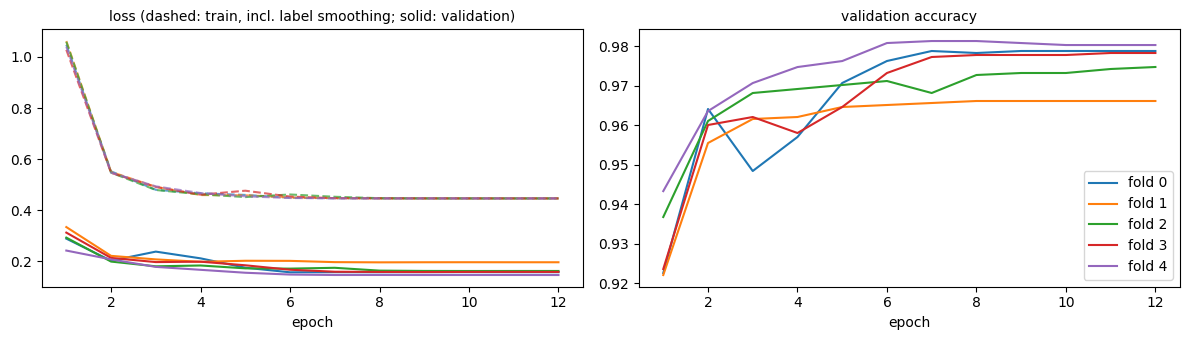
\includegraphics[width=\textwidth]{figures/training_curves.png}
  \caption{Left: training loss (dashed, includes label smoothing) and validation loss (solid) per fold.
  Right: validation accuracy per epoch.}
  \label{fig:curves}
\end{figure}

Thanks to the pretraining, validation accuracy is above 92\,\% after the first epoch and above 95\,\%
after the second (Figure~\ref{fig:curves}). It levels off around epoch 7--8, when the cosine schedule has
brought the learning rate close to zero. The validation loss never rises, so 12 epochs do not over-fit,
even though the training loss reaches its floor of $\approx0.446$. The training time is about 16\,s per
epoch, i.e.\ 17.4 minutes for the 5 folds on an NVIDIA RTX 4070 Laptop GPU.

\subsection{Per-class performance and confusion matrix}

\begin{table}[H]
\centering\small
\caption{Per-vendor out-of-fold precision, recall and F1.}
\label{tab:perclass}
\begin{tabular}{l S[table-format=1.4] S[table-format=1.4] S[table-format=1.4] S[table-format=4.0]}
\toprule
\textbf{Vendor} & {\textbf{Precision}} & {\textbf{Recall}} & {\textbf{F1}} & {\textbf{Images}} \\
\midrule
\vendor{apple}     & 0.9400 & 0.9766 & 0.9579 & 1924 \\
\vendor{facebook}  & 0.9884 & 0.9682 & 0.9782 & 1667 \\
\vendor{google}    & 0.9732 & 0.9867 & 0.9799 & 1877 \\
\vendor{messenger} & 0.9777 & 0.9828 & 0.9802 & 580 \\
\vendor{mozilla}   & 0.9796 & 0.9698 & 0.9747 & 397 \\
\vendor{samsung}   & 0.9887 & 0.9804 & \bfseries 0.9846 & 1790 \\
\vendor{whatsapp}  & 0.9937 & 0.9629 & 0.9781 & 1644 \\
\midrule
Macro average      & 0.9773 & 0.9753 & 0.9762 & 9879 \\
\bottomrule
\end{tabular}
\end{table}

% helper for the confusion matrix: shade a cell
\newcommand{\cmc}[2]{\cellcolor{accent!#1}#2}
\begin{table}[H]
\centering\small
\caption{Out-of-fold confusion matrix (rows: true vendor, columns: predicted vendor). Off-diagonal cells
with at least 5 errors are shaded. The \vendor{apple} column collects 120 of the 241 errors.}
\label{tab:cm}
\setlength{\tabcolsep}{5pt}
\begin{tabular}{l|ccccccc}
\toprule
\textbf{true} $\backslash$ \textbf{pred.} & \vendor{apple} & \vendor{facebook} & \vendor{google} & \vendor{messenger} & \vendor{mozilla} & \vendor{samsung} & \vendor{whatsapp} \\
\midrule
\vendor{apple}     & \cmc{35}{\textbf{1879}} & \cmc{12}{6} & \cmc{40}{25} & 0 & 1 & \cmc{20}{10} & 3 \\
\vendor{facebook}  & \cmc{50}{33} & \cmc{35}{\textbf{1614}} & \cmc{12}{7} & \cmc{12}{6} & 1 & 0 & \cmc{12}{6} \\
\vendor{google}    & \cmc{35}{21} & 1 & \cmc{35}{\textbf{1852}} & 0 & 1 & 2 & 0 \\
\vendor{messenger} & 0 & 4 & 1 & \cmc{35}{\textbf{570}} & \cmc{10}{5} & 0 & 0 \\
\vendor{mozilla}   & 1 & 1 & 3 & \cmc{12}{7} & \cmc{35}{\textbf{385}} & 0 & 0 \\
\vendor{samsung}   & \cmc{45}{28} & 0 & \cmc{12}{6} & 0 & 0 & \cmc{35}{\textbf{1755}} & 1 \\
\vendor{whatsapp}  & \cmc{55}{37} & \cmc{12}{7} & \cmc{15}{9} & 0 & 0 & \cmc{15}{8} & \cmc{35}{\textbf{1583}} \\
\bottomrule
\end{tabular}
\end{table}

\noindent Three patterns stand out (Table~\ref{tab:cm}):
\begin{itemize}
  \item \textbf{``Apple'' is the default answer when the model is unsure.} Half of all errors are
  predicted as \vendor{apple}, which gives it the lowest precision (0.940). Apple is the largest class
  and, as shown below, its native $72\times72$ format is shared with many hard images.
  \item \textbf{Facebook vs Messenger} (10 errors in the two directions): both are Meta products and share
  part of their design language.
  \item \textbf{Messenger vs Mozilla} (12 errors in the two directions): two flat, $240\times240$ styles, and the two smallest
  classes.
\end{itemize}

\subsection{Where do the errors come from?}

Most vendors deliver almost all their emojis at one ``usual'' size (Table~\ref{tab:data}), but a few
hundred images come at another, usually smaller, size. Table~\ref{tab:offsize} compares the two groups.

\begin{table}[H]
\centering\small
\caption{OOF accuracy by native size. Top: images at their vendor's usual size vs.\ the others. Bottom:
detail of the vendor/size combinations with at least 5 images.}
\label{tab:offsize}
\begin{tabular}{l l r r r}
\toprule
\textbf{Group} & & \textbf{Images} & \textbf{Accuracy (\%)} & \textbf{Errors} \\
\midrule
Vendor's usual size & & 9430 & 98.6 & 133 \\
Other size          & & 449  & \textbf{76.0} & 108 \\
\midrule
\textbf{Vendor} & \textbf{Native size} & & & \\
\vendor{facebook} & $240\times240$ (usual) & 1550 & 99.2 & \\
                  & $72\times72$           & 117  & \down{65.0} & \\
\vendor{whatsapp} & $160\times160$ (usual) & 1484 & 99.7 & \\
                  & $72\times72$           & 147  & \down{65.3} & \\
                  & $64\times64$           & 13   & \down{53.8} & \\
\vendor{mozilla}  & $240\times240$ (usual) & 362  & 97.8 & \\
                  & $72\times72$           & 35   & \down{88.6} & \\
\vendor{samsung}  & $72\times72$ (usual)   & 1784 & 98.2 & \\
                  & $108\times108$         & 6    & \down{50.0} & \\
\vendor{google}   & $72\times72$ (usual)   & 1756 & 98.6 & \\
                  & $72\times68$           & 116  & \up{100.0} & \\
\bottomrule
\end{tabular}
\end{table}

The model is very accurate on images at their vendor's usual size (98.6\,\%), but much weaker on the
``off-size'' ones (76.0\,\%). They are \textbf{4.5\,\% of the data but 45\,\% of the errors}. At 72\,px much
of the fine detail that separates vendors is gone. Moreover, $72\times72$ is precisely the usual size of
\vendor{apple}, \vendor{google} and \vendor{samsung}, so a small Facebook or WhatsApp emoji is mostly
predicted as one of those three, which explains the \vendor{apple} column of the confusion matrix. Only a
few dozen to about 150 training examples per vendor exist at those sizes. Google's $72\times68$ images
are the exception: they are almost the same size as the usual $72\times72$ and are classified perfectly.

\begin{figure}[tbp]
  \centering
  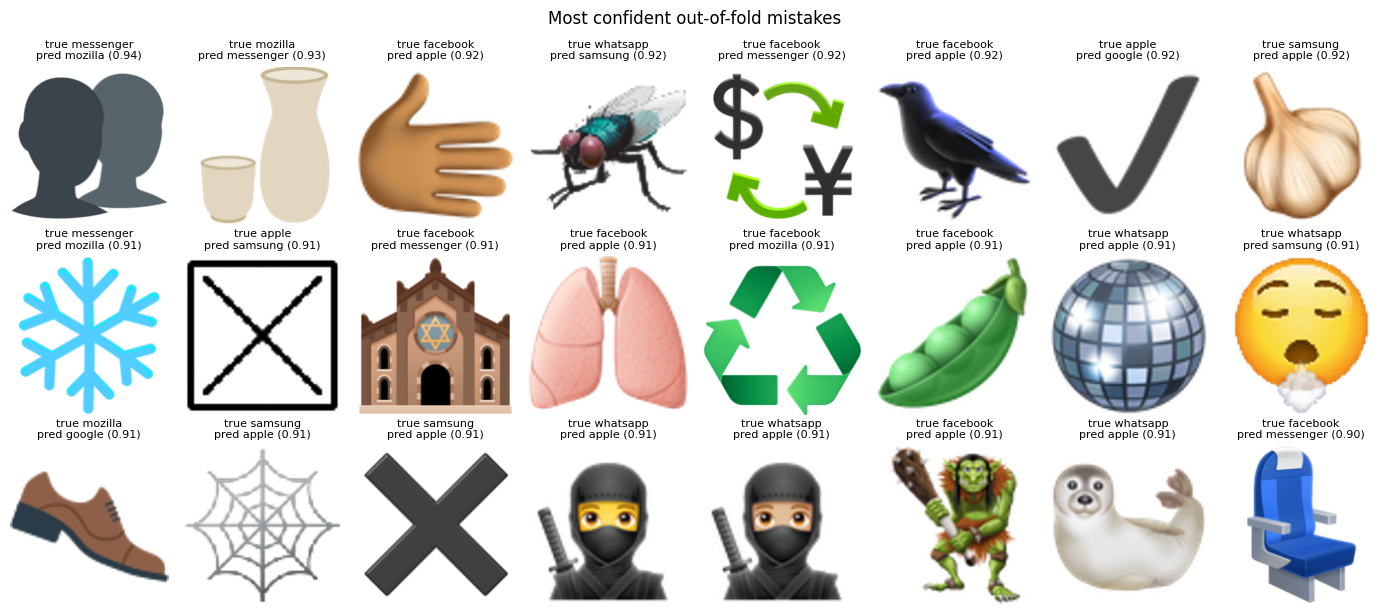
\includegraphics[width=\textwidth,trim=0 0 0 30,clip]{figures/confident_mistakes.png}
  \caption{The 24 most confident out-of-fold mistakes (true vendor, predicted vendor and probability).
  Many are blurry upscaled small images, or simple symbols (check mark, cross, snowflake) that carry
  little vendor-specific style.}
  \label{fig:mistakes}
\end{figure}

\subsection{Ablation study}
\label{sec:ablation}

To check that each design choice is useful, we changed \textbf{one} element of the final recipe at a time
and retrained on fold 0 with the same seed, epochs and optimiser (Table~\ref{tab:ablation}). A fold has
\num{1976} validation images, so one image is worth 0.05 accuracy points, and differences of a few tenths
of a point (5 to 8 images) are within the noise between splits and seeds.

\begin{table}[H]
\centering\small
\caption{Ablation on fold 0 (\num{1976} validation images).}
\label{tab:ablation}
\begin{tabular}{l r r r}
\toprule
\textbf{Variant} & \textbf{Accuracy (\%)} & \textbf{$\Delta$ (pts)} & \textbf{Macro-F1} \\
\midrule
\textbf{Final recipe} (premultiplied alpha, no augmentation) & \textbf{97.87} & -- & \textbf{0.9799} \\
+ geometric augmentation (rotation, zoom, translation) & 95.14 & \down{$-2.73$} & 0.9537 \\
+ horizontal flip (training + test-time)               & 97.47 & $-0.40$ & 0.9754 \\
Naive \code{convert("RGB")} instead of premultiplied alpha & 97.82 & $-0.05$ & 0.9776 \\
\bottomrule
\end{tabular}
\end{table}

\begin{figure}[H]
\centering
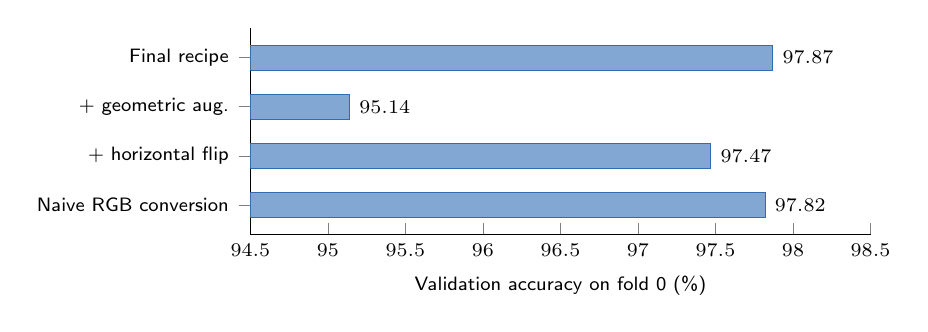
\begin{tikzpicture}
\begin{axis}[
  xbar, width=0.78\textwidth, height=4.2cm,
  xmin=94.5, xmax=98.5,
  xlabel={Validation accuracy on fold 0 (\%)},
  symbolic y coords={final,geo,flip,naive},
  ytick={final,geo,flip,naive},
  yticklabels={Final recipe,+ geometric aug.,+ horizontal flip,Naive RGB conversion},
  y dir=reverse,
  bar width=9pt,
  nodes near coords, nodes near coords style={font=\scriptsize},
  tick label style={font=\scriptsize\sffamily}, label style={font=\scriptsize\sffamily},
  axis lines*=left, enlarge y limits=0.2]
\addplot[fill=accent!60,draw=accent] coordinates {(97.87,final) (95.14,geo) (97.47,flip) (97.82,naive)};
\end{axis}
\end{tikzpicture}
\caption{Ablation results. Only geometric augmentation has an effect larger than the noise, and it is
negative.}
\label{fig:ablation}
\end{figure}

\begin{itemize}
  \item \textbf{Geometric augmentation: $-2.7$ points}, a clear loss (it was also the largest effect in
  our preliminary experiments).
  \item \textbf{Horizontal flip (+ flip TTA): $-0.4$ points} here, but $+0.4$ points in a preliminary
  experiment on another split. Over the full 5-fold cross-validation the two recipes are equivalent
  (97.52\,\% vs 97.56\,\% OOF accuracy), so we keep the simpler pipeline.
  \item \textbf{Naive RGB conversion: $-0.05$ points}, i.e.\ the same score. The network does not need the
  hidden colours to reach this accuracy. The clean preprocessing costs nothing and guarantees that the
  model only uses what is actually visible.
\end{itemize}

\subsection{Test predictions}

The 5 fold models are averaged on the test set. Of the 352 test images that are identical to a training
image, the ensemble already predicted the correct training label for all 352, so the duplicate lookup
changes \textbf{0} predictions. It acts as a safety net and as an independent check of the model. The
predicted class distribution on the test set is very close to the training distribution
(Table~\ref{tab:testdist}), which suggests the test set is drawn from the same distribution. Only 64
test images have a maximum predicted probability below 0.5.

\begin{table}[H]
\centering\small
\caption{Class shares in the training labels and in our test predictions (\code{submission.csv}).}
\label{tab:testdist}
\begin{tabular}{l *{7}{S[table-format=2.1]}}
\toprule
 & {\vendor{apple}} & {\vendor{facebook}} & {\vendor{google}} & {\vendor{messenger}} & {\vendor{mozilla}} & {\vendor{samsung}} & {\vendor{whatsapp}} \\
\midrule
Training share (\%)       & 19.5 & 16.9 & 19.0 & 5.9 & 4.0 & 18.1 & 16.6 \\
Test predicted share (\%) & 19.6 & 15.9 & 19.6 & 6.1 & 4.2 & 18.3 & 16.3 \\
\bottomrule
\end{tabular}
\end{table}

% ============================ AI AND CODE ============================
\section{AI and Code}
\label{sec:code}

\subsection{Code organisation}

The whole solution is a single Jupyter notebook, \code{emoji\_classifier.ipynb}, that runs top to
bottom and writes every result to disk. Table~\ref{tab:code} maps its sections to this report.

\begin{table}[H]
\centering\small
\caption{Structure of the notebook and of the repository.}
\label{tab:code}
\begin{tabularx}{\textwidth}{@{}l X l@{}}
\toprule
\textbf{Notebook section} & \textbf{Content and main functions} & \textbf{Report} \\
\midrule
0. Setup        & package versions, \code{CFG} dictionary, \code{seed\_everything} & \S\ref{sec:archi} \\
1. The data     & class balance, native sizes and PNG modes, sample grid & \S\ref{sec:prepro} \\
2. Preprocessing & \code{load\_premultiplied}, \code{load\_folder}, \code{composite\_on\_white}; fingerprints, duplicates, \code{StratifiedGroupKFold} folds; near-duplicate check with perceptual hashes (added later, not executed yet) & \S\ref{sec:prepro} \\
3. Baseline     & metadata-only decision tree & \S\ref{sec:prepro} \\
4. Model and training & \code{normalize}, \code{augment}, \code{predict\_proba}, \code{train\_one\_fold}; 5-fold loop & \S\ref{sec:archi} \\
5. Evaluation   & OOF metrics, learning curves, confusion matrix, error analysis & \S\ref{sec:perf} \\
6. Submission   & fold averaging, duplicate lookup, format checks, \code{submission.csv} & \S\ref{sec:perf} \\
7. Ablation     & one-change-at-a-time variants on fold 0 & \S\ref{sec:ablation} \\
8. Experiments  & oversampling of the off-size images, nearest-neighbour upscaling, 8 epochs, final model retrained on 100\,\% of the data with 3 seeds (added later, not executed yet) & \S\ref{sec:conclusion} \\[2pt]
9. Summary      & results and lessons & \S\ref{sec:conclusion} \\
\bottomrule
\end{tabularx}
\end{table}

\noindent Besides the notebook, the repository contains \code{requirements.txt} (pinned package versions),
the training history and ablation results (\code{outputs/history.csv}, \code{outputs/ablation.csv}), the
out-of-fold and test probabilities (\code{outputs/oof\_proba.npy}, \code{outputs/test\_proba.npy}), the
final \code{submission.csv}, a \code{README.md} with setup and running instructions, and
\code{AI\_USAGE.md}, the declaration of AI assistance (Section~\ref{sec:ai}).

\paragraph{Implementation choices.}
\begin{itemize}
  \item \textbf{One configuration dictionary.} Every helper takes a \code{cfg} argument, so the same code
  trains the final model and each ablation variant (e.g.\ \code{dict(CFG, geometric\_aug=True)}).
  \item \textbf{In-memory, GPU-side pipeline.} The preprocessed images are kept as \code{uint8} tensors
  (about 1\,GB per split), and compositing, normalisation and augmentation run on the GPU per batch.
  There is no disk cache and no \code{DataLoader} worker, which also avoids multiprocessing problems with
  Jupyter on Windows.
  \item \textbf{Built-in checks.} The code asserts that no fingerprint is shared between the training and
  validation parts of a fold, that duplicates never disagree on their label, and that the submission has
  one row per test file, in order, with valid labels only.
  \item \textbf{Hardware independence.} Mixed precision uses bfloat16 on recent GPUs and falls back to
  float16 with gradient scaling otherwise (e.g.\ a Kaggle T4), or to the CPU.
\end{itemize}

The core of the training loop is short:
\begin{lstlisting}
for k in range(steps_per_epoch):
    idx = perm[k * bs:(k + 1) * bs]
    img = augment(composite_on_white(X[idx]), cfg)        # uint8 premultiplied RGBA -> RGB on white
    target = y_t[idx].to(DEVICE)
    with torch.autocast(DEVICE.type, dtype=AMP_DTYPE, enabled=USE_AMP):
        loss = F.cross_entropy(model(normalize(img, model)), target,
                               label_smoothing=cfg["label_smoothing"])
    opt.zero_grad(set_to_none=True)
    scaler.scale(loss).backward()
    scaler.step(opt); scaler.update(); sched.step()
\end{lstlisting}

\subsection{Reproducibility}
All random seeds (Python, NumPy, PyTorch CPU and GPU) are fixed, cuDNN is forced to deterministic
algorithms, and \code{CUBLAS\_WORKSPACE\_CONFIG} is set before CUDA is initialised. Two complete,
independent runs of the notebook gave identical losses and accuracies at every epoch. The exact package
versions are pinned in \code{requirements.txt} (Python 3.12, PyTorch 2.11 with CUDA 12.8, \code{timm}
1.0.30, scikit-learn 1.9.1), and the pretrained weights are downloaded from a fixed Hugging Face Hub
commit, so the starting point of the fine-tuning cannot change. On an RTX 4070 Laptop GPU the full run takes about 2 minutes of image
loading, 18 minutes of 5-fold training and 11 minutes of ablation.

\subsection{Use of AI tools}
\label{sec:ai}

We used an AI coding assistant, \textbf{Claude Code} (Anthropic) with the \textbf{Claude Opus 5.5}
model. Starting from the competition rules, it designed, wrote and ran the notebook on our GPU,
including the exploratory hyperparameter sweep and the ablation study, and it drafted this report from
the notebook's outputs. The repository records this: the commits that add the notebook and the report
list Claude as a co-author, and \code{AI\_USAGE.md} declares the tools used, the AI-assisted files and
notebook cells, how each of them was checked, and every prompt sent to the assistant.

We kept the following rules so that the results can be trusted:
\begin{itemize}
  \item \textbf{Every claim is backed by an executed cell.} All the numbers in this report come from the
  outputs stored in the notebook and in \code{outputs/}, not from the assistant's expectations.
  \item \textbf{Defaults are tested, not assumed.} The ``standard recipe'' for small image datasets
  includes data augmentation; our ablation showed that, here, it costs 2.7 points. Likewise, the
  premultiplied-alpha preprocessing was kept because it removes a shortcut, and the ablation confirmed
  that it costs nothing.
  \item \textbf{Validation is protected against leaks.} Duplicate-aware folds and assertions make sure
  the reported scores are not inflated, whoever wrote the code.
  \item \textbf{Understanding before submitting.} Each step of the pipeline is explained in the notebook
  and in this report, and we can justify every hyper-parameter in Table~\ref{tab:hyper}.
\end{itemize}

% ============================ CONCLUSION ============================
\section{Conclusion}
\label{sec:conclusion}

We built a vendor classifier for emojis that reaches \textbf{97.56\,\%} out-of-fold accuracy and a
macro-F1 of \textbf{0.976}, with a ConvNeXt-Tiny CNN fine-tuned from ImageNet-22k weights and averaged
over 5 folds; its submission scores \textbf{\kagglepublic} on the Kaggle public leaderboard. Four
lessons stand out:
\begin{enumerate}
  \item \textbf{Careful decoding matters more than model size.} Converting every PNG mode to premultiplied
  RGBA, padding, resizing and compositing on white gives clean and comparable inputs, and removes the
  hidden-colour shortcut at no cost in accuracy.
  \item \textbf{Validation must be honest.} Exact duplicates (141 groups) are kept inside one fold, so the
  OOF score is a reliable estimate; the 352 test images identical to a training image were all already
  predicted correctly.
  \item \textbf{Augmentation is not always helpful.} When the class is a rendering style, geometric
  transformations destroy the signal ($-2.7$ points).
  \item \textbf{The remaining errors have a clear cause.} Images delivered at an unusual small size are
  4.5\,\% of the data but 45\,\% of the errors, mostly predicted as one of the $72\times72$ vendors.
\end{enumerate}

\paragraph{Limitations and next steps.} The main limitation is the low resolution of the ``off-size''
images. Section~8 of the notebook, added after the results of this report, tests two remedies:
over-sampling the off-size images during training and upscaling small images with nearest-neighbour
interpolation instead of bicubic. It also tests a shorter 8-epoch schedule and retrains the best setup
on 100\,\% of the training data with 3 seeds; it has not been run yet. Other directions are to give the
network the native resolution as an extra input (or a dedicated branch for small images), to ensemble
different backbones (e.g.\ a ConvNeXt with an EfficientNet), and to pseudo-label the most confident test
predictions.

% ============================ REFERENCES ============================
\begin{thebibliography}{9}\small
\bibitem{liu2022convnext}
Z.~Liu, H.~Mao, C.-Y.~Wu, C.~Feichtenhofer, T.~Darrell, S.~Xie.
\newblock A ConvNet for the 2020s.
\newblock \emph{CVPR}, 2022.

\bibitem{deng2009imagenet}
J.~Deng, W.~Dong, R.~Socher, L.-J.~Li, K.~Li, L.~Fei-Fei.
\newblock ImageNet: A large-scale hierarchical image database.
\newblock \emph{CVPR}, 2009.

\bibitem{porter1984compositing}
T.~Porter, T.~Duff.
\newblock Compositing digital images.
\newblock \emph{SIGGRAPH}, 1984.

\bibitem{loshchilov2019adamw}
I.~Loshchilov, F.~Hutter.
\newblock Decoupled weight decay regularization.
\newblock \emph{ICLR}, 2019.

\bibitem{smith2019superconvergence}
L.~N.~Smith, N.~Topin.
\newblock Super-convergence: very fast training of neural networks using large learning rates.
\newblock \emph{Artificial Intelligence and Machine Learning for Multi-Domain Operations Applications}, SPIE, 2019.

\bibitem{szegedy2016rethinking}
C.~Szegedy, V.~Vanhoucke, S.~Ioffe, J.~Shlens, Z.~Wojna.
\newblock Rethinking the Inception architecture for computer vision.
\newblock \emph{CVPR}, 2016.

\bibitem{wightman2019timm}
R.~Wightman.
\newblock PyTorch Image Models (\code{timm}).
\newblock \url{https://github.com/huggingface/pytorch-image-models}, 2019.
\end{thebibliography}

\end{document}
